\chapter{Алгоритм на основе нисходящего анализа}

В данном разделе мы рассмотрим семейство алгоритмов нисходящего синтаксического (рекурсивный спуск, LL, GLL~\cite{Scott:2010:GP:1860132.1860320,10.1007/978-3-662-46663-6_5}) рассмотрим их обощение для задачи поиска путей с контекстно-свободными ограничениями.

% и GLL~\cite{Grigorev:2017:CPQ:3166094.3166104} Другие реализации~\cite{MEDEIROS201975}

\section{Рекурсивный спуск}

Идея рекурсивного спуска основана на использовании программного стека вызовов в качестве стека магазинного автомата. Достигается это следующим образом.
\begin{itemize}
  \item Для каждого нетерминала создаётся функция, принимающая ещё не обработанный остаток строки и возвращающая пару: результат вывода префикса данной строки из соответствующего нетерминала и не обработанный остаток строки. В случае распознавателя результат вывода --- логическое значение (выводится/не выводится).
  \item Каждая такая функция реализовывает обработку цепочки согласно правым частям правил для соответствующих нетерминалов: считывание символа входа при обработке терминального символа, вызов соответствующей функции при обработке нетерминального.
\end{itemize}

У такого подхода есть два ограничения:
\begin{enumerate}
  \item Не работает с леворекурсивными грамматиками, грамматиками, в которых вывод может принимать следующий вид:
  $$
  S \to \cdots \to \underline{N_i} \alpha \to \cdots \underline{N_i} \beta \to \cdots \omega
  $$
  \item Шаги должны быть однозначными.
\end{enumerate}

\begin{example}

Построим функцию рекурсивного спуска для продукции $S \rightarrow aSbS \mid \varepsilon$.

\begin{algorithm}
  \floatname{algorithm}{Listing}
\begin{algorithmic}[1]
\caption{Функция рекурсивного спуска}
\Function{S}{$\omega$}
    \If {(len$(\omega)=0$)}
    \Comment{{\footnotesize Пустая цепочка выводима из $S$}}
    \State{\Return \textit{(true, $\omega$)}}
    \EndIf

    \If{$(\omega = a :: tl)$}
        \Comment{{\footnotesize Выводимая из $S$ подстрока должна начинаться с $a$}}
        \State{$res,tl' = $ S($tl$)}
        \Comment{{\footnotesize Затем должна идти подстрока, выводимая из $S$}}
        \If{res \&\&  $tl' = b :: tl''$}
           \Comment{{\footnotesize Если вызов закончился успешно, то надо проверить, что следующий символ --- это $b$}}
           \State{\Return $S(tl'')$}
           \Comment{{\footnotesize И снова попробовать вывести перфикс из $S$}}
         \Else
           \State{\Return \textit{(false, $tl'$)}}
        \EndIf
    \Else
        \State{\Return \textit{(false, $\omega$)}}
    \EndIf
\EndFunction

\end{algorithmic}
\end{algorithm}
\end{example}

Если возвращаеммое значение этой функции  --- пара вида \textit{(true, [])}, то разбор завершился успехом.

Данный подход применяется как для ручного написания синтаксических нализаторов, так и при генерации анализаторов по грамматике.

\section{LL(k)-алгоритм синтаксического анализа}

LL(k) --- алгоритм синтаксического анализа --- нисходящий анализ без отката, но с предпросмотром.
Решение о том, какую продукцию применять, принимается на основании k следующих за текущим символом.
Временная сложность алгоритма $O(n)$, где $n$~--- длина слова.

Алгоритм использует входной буфер, стек для хранения промежуточных данных и таблицу анализатора, которая управляет процессом разбора.
В ячейке таблицы указано правило, которое нужно применять, если рассматривается нетерминал $A$, а следующие $m$ символов строки~--- $t_{1} \dots t_{m}$, где $m \leq k$.
Также в таблице выделена отдельная колонка для $\$$~--- маркера конца строки.

\begin{center}
  \begin{tabular}{ c || c | c | c | c }
             & $\dots$ & $t_{1} \dots t_{m}$ & $\dots$ & $\$$ \\ \hline
    $\dots$  & $\dots$ & $\dots$ & $\dots$ & $\dots$ \\ \hline
    $A$  & $\dots$ & $A \to \alpha$ & $\dots$ & $\dots$ \\ \hline
    $\dots$  & $\dots$ & $\dots$ & $\dots$ & $\dots$
  \end{tabular}
\end{center}

Для построения таблицы вычисляются множества $\first[k]$ и $\follow[k]$. Идейно их можно понимать, как первые или, соответственно, последующие $k$ символов в результирующем выводе, при использовании нетерминала $A$. Данную мысль хорошо иллюстрирует рисунок:

\begin{center}
    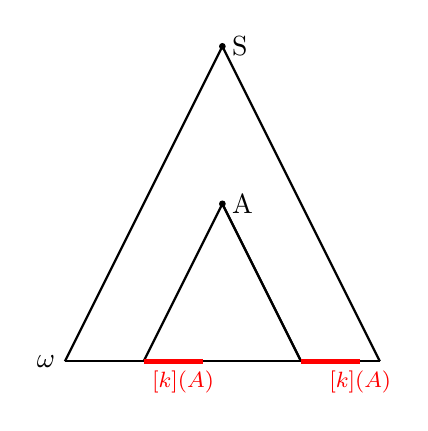
\begin{tikzpicture}
        \draw[black, thick] (0,0) -- (2,4);
        \draw[black, thick] (2,4) -- (4,0);
        \draw[black, thick] (1,0) -- (2,2);
        \draw[black, thick] (2,2) -- (3,0);
        \draw[black, thick] (2,2) -- (3,0);
        \draw[black, thick] (0,0) -- (1,0);
        \draw[red, ultra thick] (1,0) -- (1.75,0);
        \draw[black, thick] (1.75,0) -- (3,0);
        \draw[red, ultra thick] (3,0) -- (3.75,0);
        \draw[black, thick] (3.75,0) -- (4,0);
        \filldraw[black] (2,4) circle (1pt) node[anchor=west] {S};
        \filldraw[black] (2,2) circle (1pt) node[anchor=west] {A};
        \filldraw[black] (0,0) circle (0pt)
        node[anchor=east] {\textbf{$\omega$}};
        \filldraw[red] (1.5,0) circle (0pt)
        node[anchor=north] {\footnotesize $\first[k](A)$};
        \filldraw[red] (3.75,0) circle (0pt)
        node[anchor=north] {\footnotesize $\follow[k](A)$};
    \end{tikzpicture}
\end{center}

Определим их формально:

\begin{definition}
  Пусть $G = \langle N, \Sigma, P, S \rangle$~--- КС-грамматика. Множество $\first[k]$ определено для сентенциальной формы $\alpha$ следующим образом:
  \[ \first[k](\alpha) = \{ \omega \in \Sigma^* \mid \alpha \derives{} \omega \text{ и } |\omega| < k \text{ либо } \exists \beta: \alpha \derives{} \omega \beta \text{ и } |\omega| = k \}
  \]
  , где $\alpha, \beta \in (N \cup \Sigma)^*.$
\end{definition}

\begin{definition}
  Пусть $G = \langle N, \Sigma, P, S \rangle$~--- КС-грамматика. Множество $\follow[k]$ определено для сентенциальной формы $\beta$ следующим образом:
  \[\follow[k](\beta) = \{ \omega \in \Sigma^* \mid \exists \gamma, \alpha: S \derives{} \gamma \beta \alpha \text{ и } \omega \in \first[k](\alpha) \} \]
\end{definition}

В частном случае для $k = 1$:

\[ \first(\alpha) = \{ a \in \Sigma \mid \exists \gamma \in (N \cup \Sigma)^*: \alpha \derives{} a \gamma \} \text{, где } \alpha \in (N \cup \Sigma)^* \]

\[ \follow(\beta) = \{ a \in \Sigma \mid \exists \gamma, \alpha \in (N \cup \Sigma)^* : S \derives{} \gamma \beta a \alpha \} \text{, где } \beta \in (N \cup \Sigma)^*  \]

Множество $\first$ можно вычислить, пользуясь следующими соотношениями:

\begin{itemize}
  \item $\first(a \alpha) = \{a\}, a \in \Sigma, \alpha \in (N \cup \Sigma)^* $
  \item $\first(\varepsilon) = \{\varepsilon\}$
  \item $\first(\alpha \beta) = \first(\alpha) \cup (\first(\beta) \text{, если } \varepsilon \in \first(\alpha))$
  \item $\first(A) = \first(\alpha) \cup \first(\beta) \text{, если в грамматике есть правило } A \to \alpha \mid\beta$
\end{itemize}

Алгоритм для вычисления множества $\follow$:

\begin{itemize}
  \item Положим $\follow(X) = \varnothing, \forall X \in N$
  \item $\follow(S) = \follow(S) \cup \{\$\} \text{, где } S \text{--- стартовый нетерминал}$
  \item Для всех правил вида $A \to \alpha X \beta: \follow(X) = \follow(X) \cup (\first(\beta) \setminus \{\varepsilon\} )$
  \item Для всех правил вида $A \to \alpha X \text{ и } A \to \alpha X \beta \text{, где } \varepsilon \in \first(\beta): \follow(X) = \follow(X) \cup \follow(A)$
  \item Последние два пункта применяются пока есть что добавлять в строящиеся множества.
\end{itemize}


\begin{example}

Рассмотрим грамматику $G$ со следующими продукциями:
\begin{align*}
  S  &\to a S' & A' \to b \mid a \\
  S' &\to A b B S' \mid \varepsilon &  B  \to c \mid \varepsilon\\
  A  &\to a A' \mid \varepsilon
\end{align*}


Пример множеств $\first$ для нетерминалов грамматики $G$:

\begin{multicols}{2}

\columnbreak

\begin{align*}
  \first(S)  &= \{ a \}  & \first(B)  &= \{ c, \varepsilon \} \\
  \first(A)  &= \{ a, \varepsilon \} & \first(S') &= \{ a, b, \varepsilon \}\\
  \first(A') &= \{ a, b \}
\end{align*}
\end{multicols}

Пример множеств $\follow$ для нетерминалов грамматики $G$:

\begin{align*}
  \follow(S)  &= \{ \$ \} & \\
  \follow(S') &= \{ \$ \} &(S \to a S')\\
  \follow(A)  &= \{ b \}  &(S' \to A b B S') \\
  \follow(A') &= \{ b \}  &(A \to a A')\\
  \follow(B)  &= \{ a, b, \$ \} &(S' \to A b B S', \varepsilon \in \first(S'))
\end{align*}

\end{example}

Управляющая таблица LL(k) анализатора заполняется следующим образом: продукции $A \to \alpha, \alpha \neq \varepsilon$ помещаются в ячейки $(A, a)$, где $a \in \first(\alpha)$, продукции $A \to \alpha$~--- в ячейки $(A, a)$, где $a \in \follow(A)$, если $\varepsilon \in \first(\alpha)$

\begin{example}

Пример таблицы для грамматики $S \to aSbS \mid \varepsilon$

\begin{center}
\begin{tabular}{ r || c | c || c | c | c }
N & $\first$ & $\follow$ & a & b & $\$ $ \\ \hline
$S$ & $\{ a, \varepsilon \}$ & $\{ b, \$ \}$ & $S \rightarrow aSbS$ & $S \rightarrow \varepsilon$ & $S \rightarrow \varepsilon$
\end{tabular}
\end{center}

\end{example}

Однако, не для всех грамматик по множествам $\first[k]$ и $\follow[k]$ возможно выбрать применяемую продукцию, а значит, нельзя однозначно построить таблицу, необходимую для работы алгоритма, поэтому данный алгоритм применим только для грамматик особого класса --- LL(k).

\begin{definition}
  LL(k) грамматика --- грамматика, для которой на основании множеств $\first[k]$ и $\follow[k]$ можно однозначно определить, какую продукцию применять.
\end{definition}

Важно заметить, что при больших $k$ управляющая таблица сильно разрастается, поэтому на практике данный алгоритм применим для небольших значений $k$.

Интерпретатор автомата принимает входную строку и построенную управляющую таблицу и работает следующим образом.
В каждый момент времени конфигурация автомата это позиция во входной строке и стек.
В начальный момент времени стек пуст, а позиция во входной строке соответствует её началу.
На первом шаге в стек добавляются последовательно сперва символ концы строки, затем стартовый нетерминал.
На каждом шаге анализируется существующая конфигурация и совершается одно из действий.
\begin{itemize}
\item Если текущая позиция --- конец строки и вершина стека --- символ конца строки, то успешно завершаем разбор.
\item Если текущая вершина стека --- терминал, то проверяем, что позиция в строке соответствует этому терминалу. Если да, то снимаем элемент со стека, сдвигаем позицию на единицу и продолжаем разбор. Иначе завершаем разбор с ошибкой.
\item Если текущая вершина стека --- нетерминал $N_i$ и текущий входной символ $t_j$, то ищем в управляющей таблице ячейку с координатами $(N_i, t_j)$ и записываем на стек содержимое этой ячейки.
\end{itemize}

\begin{example}Пример работы LL анализатора.
Рассмотрим грамматику $S \to aSbS \mid \varepsilon$ и выводимое слово $\omega = abab$.

Расмотрим пошагово работу алгоритма, будем использовать таблицу, построенную в предыдущем примере:

\begin{enumerate}
  \item Начало работы.

  Стек: \,
    \begin{tabular}[c]{ |c| }
        \\ \hline
        \$ \\ \hline
    \end{tabular}
    \qquad  \qquad \qquad  \qquad входное слово: \,
    \begin{tabular}[c]{ |c|c|c|c|c| }
        \hline
        \textcolor{red}{a} & b & a & b & \$ \\ \hline
    \end{tabular}

Финальный символ лежит на стеке, а указатель указывает на первый символ слова.

  \item кладем стартовый символ на стек

    Стек: \,
    \begin{tabular}[c]{ |c| }
        \\ \hline
        $S$ \\ \hline
        \$ \\ \hline
    \end{tabular}
    \qquad  \qquad \qquad  \qquad входное слово: \,
    \begin{tabular}[c]{ |c|c|c|c|c| }
        \hline
        \textcolor{red}{a} & b & a & b & \$ \\ \hline
    \end{tabular}

  \item Ищем ячейку с координатами (S, a), применяем продукцию из ячейки.

    Стек: \,
    \begin{tabular}[c]{ |c| }
        \\ \hline
        $a$ \\ \hline
        $S$ \\ \hline
        $b$ \\ \hline
        $S$ \\ \hline
        \$ \\ \hline
    \end{tabular}
    \qquad  \qquad \qquad  \qquad входное слово: \,
    \begin{tabular}[c]{ |c|c|c|c|c| }
        \hline
        \textcolor{red}{a} & b & a & b & \$ \\ \hline
    \end{tabular}

\item Снимаем терминал $a$ со стека и двигаем указатель.

    Стек: \,
    \begin{tabular}[c]{ |c| }
        \\ \hline
        $S$ \\ \hline
        $b$ \\ \hline
        $S$ \\ \hline
        \$ \\ \hline
    \end{tabular}
    \qquad  \qquad \qquad  \qquad входное слово: \,
    \begin{tabular}[c]{ |c|c|c|c|c| }
        \hline
        a & \textcolor{red}{b} & a & b & \$ \\ \hline
    \end{tabular}

\item Ищем ячейку с координатами (S, b), применяем продукцию из ячейки.

    Стек: \,
    \begin{tabular}[c]{ |c| }
        \\ \hline
        $b$ \\ \hline
        $S$ \\ \hline
        \$ \\ \hline
    \end{tabular}
    \qquad  \qquad \qquad  \qquad входное слово: \,
    \begin{tabular}[c]{ |c|c|c|c|c| }
        \hline
        a & \textcolor{red}{b} & a & b & \$ \\ \hline
    \end{tabular}

\item Снимаем терминал $b$ со стека и двигаем указатель.

    Стек: \,
    \begin{tabular}[c]{ |c| }
        \\ \hline
        $S$ \\ \hline
        \$ \\ \hline
    \end{tabular}
    \qquad  \qquad \qquad  \qquad входное слово: \,
    \begin{tabular}[c]{ |c|c|c|c|c| }
        \hline
        a & b & \textcolor{red}{a} & b & \$ \\ \hline
    \end{tabular}

  \item Ищем ячейку с координатами (S, a), применяем продукцию из ячейки.

    Стек: \,
    \begin{tabular}[c]{ |c| }
        \\ \hline
        $a$ \\ \hline
        $S$ \\ \hline
        $b$ \\ \hline
        $S$ \\ \hline
        \$ \\ \hline
    \end{tabular}
    \qquad  \qquad \qquad  \qquad входное слово: \,
    \begin{tabular}[c]{ |c|c|c|c|c| }
        \hline
        a & b & \textcolor{red}{a} & b & \$ \\ \hline
    \end{tabular}

\item Снимаем терминал $a$ со стека и двигаем указатель.

    Стек: \,
    \begin{tabular}[c]{ |c| }
        \\ \hline
        $S$ \\ \hline
        $b$ \\ \hline
        $S$ \\ \hline
        \$ \\ \hline
    \end{tabular}
    \qquad  \qquad \qquad  \qquad входное слово: \,
    \begin{tabular}[c]{ |c|c|c|c|c| }
        \hline
        a & b & a & \textcolor{red}{b} & \$ \\ \hline
    \end{tabular}

\item Ищем ячейку с координатами (S, b), применяем продукцию из ячейки.

    Стек: \,
    \begin{tabular}[c]{ |c| }
        \\ \hline
        $b$ \\ \hline
        $S$ \\ \hline
        \$ \\ \hline
    \end{tabular}
    \qquad  \qquad \qquad  \qquad входное слово: \,
    \begin{tabular}[c]{ |c|c|c|c|c| }
        \hline
        a & b & a & \textcolor{red}{b} & \$ \\ \hline
    \end{tabular}

\item Снимаем терминал $b$ со стека и двигаем указатель.

    Стек: \,
    \begin{tabular}[c]{ |c| }
        \\ \hline
        $S$ \\ \hline
        \$ \\ \hline
    \end{tabular}
    \qquad  \qquad \qquad  \qquad входное слово: \,
    \begin{tabular}[c]{ |c|c|c|c|c| }
        \hline
        a & b & a & b & \textcolor{red}{\$} \\ \hline
    \end{tabular}

\item Ищем ячейку с координатами (S, \$), применяем продукцию из ячейки.

    Стек: \,
    \begin{tabular}[c]{ |c| }
        \\ \hline
        \$ \\ \hline
    \end{tabular}
    \qquad  \qquad \qquad  \qquad входное слово: \,
    \begin{tabular}[c]{ |c|c|c|c|c| }
        \hline
        a & b & a & b & \textcolor{red}{\$} \\ \hline
    \end{tabular}

\item Оказались в конце строки и на вершине стека символ конца --- завершаем разбор.

\end{enumerate}

\end{example}

Можно расширить данный алгоритм так, чтобы он строил дерево вывода. Дерево будет строиться сверху вниз, от корня к листьям. Для этого необходимо расширить шаги алгоритма.
\begin{itemize}
  \item В ситуации, когда мы читаем очередной нетерминал (на вершине стека и во входе одинаковые терминалы), мы создаём лист с соответствующим терминалом.
  \item В ситуации, когда мы заменяем нетерминал на стеке на правую часть продукции в соответствии с управляющей таблицей, мы создаём нетерминальный узел соответствующий применяемой продукции.
\end{itemize}

Данное семейство всё так же не работает с леворекурсивными грамматиками и с неоднозначными грамматиками.

Таким образом, по некоторым граммтикам можно построить LL(k) анализатор (назовём их LL(k) граммтиками), но не по всем.
С левой рекурсией, конечно, можно бороться, так как существуют алгоритмы устранения левой и скрытой левой рекурсии, а вот с неоднозначностями ничего не поделаешь.



\section{Алгоритм Generalized LL}

Можно построить анализатор, работающий с произвольными КС-грамматиками.
Generalized LL (GLL)~\cite{Scott:2010:GP:1860132.1860320,10.1007/978-3-662-46663-6_5}

Принцип работы остается абсолютно таким же как и для табличного LL:
\begin{itemize}
  \item Сначала по грамматике строится \textit{управляющая} таблица
  \item Затем построенная таблица команд и непосредственно анализируемое слово поступают на вход абстрактному интерпретатору.
  \item Для своей работы интерпретатор поддерживает некоторую вспомогательную структуру данных (стек для LL).
  \item Один шаг разбора состоит в том, чтобы рассмотреть текущую позицию в слове, применить все соответствующие ей правила из таблицы и при возможности сдвинуть позицию разбора вправо.
\end{itemize}

Где в этой схеме возникают ограничения на вид обрабатываемой грамматики для алгоритма LL? На самом первом шаге --- при построении таблицы может возникнуть ситуация, когда одному нетерминалу $N_j$ и последовательности $first_k(N_j)$ соответствует несколько продукций грамматики. В этом случае грамматика признавалась не соответствующей классу LL(k) и отвергалась анализатором.

Теперь же мы разрешим такую ситуацию и в этом случае в ячейку таблицы будем записывать все продукции грамматики, соответствующие этой ячейке. Однако сразу же возникает вопрос --- а что делать интерпретатору, когда при разборе ему необходимо применить правило, состоящее из нескольких продукций? Общий ответ такой --- необходим некоторый вид недетерминизма, при котором интерпретатор мог бы ``параллельно'' обрабатывать несколько возможных вариантов синтаксического разбора.

Эти два свойства (модифицированная управляющая таблица и недетерминизм) суть главные принципиальные отличия GLL(k) от LL(k). Далее мы перейдем к рассмотрению непосредственно технической реализации описанного алгоритма.

Нам необходимо научиться задавать различные ветви (пути) синтаксического разбора и переключаться между ними. Заметим, что состояние любой ветви в любой момент времени суть следующее: необходимо распознать символ $N_j \in N \cup \Sigma$ из продукции $X$, начиная с элемента слова под индексом $i$. Т.е. имеем позицию в слове и позицию символа в продукции. Последнее принято называть \textit{слотом грамматики}.

\begin{definition}
  Пусть $G = \langle N, \Sigma, P, S \rangle$~--- КС-грамматика. \textit{Слотом грамматики} $G$ (позицией грамматики $G$) назовем пару из продукции $X \in P$ и позиции $0 \leq q \leq length(body(X))$ тела продукции $X$. При этом введем следующее обозначение $X ::= \alpha \cdot \beta, \quad \alpha,\beta \in (N \cup \Sigma)^*$, где $ \cdot $ указывает на позицию в продукции.
\end{definition}

Описанная пара позиций уже однозначно задает состояние синтаксического разбора. Имеем множество состояний и переходов между ними --- возникает естественное желание воспользоваться терминами графов для представления этой структуры. Такую конструкцию называют \textit{граф-структурированный стек} или \textit{GSS} (Graph Structured Stack), который впервые был предложен Масару Томитой ~\cite{tomita1988graph} в контексте восходящего анализа. GSS будет являться рабочей структурой нашего нового интерпретатора вместо стека для LL. Состояние разбора вместе с узлом GSS мы будет называть \textit{дескриптором}.

\begin{definition}
  Пусть $G = \langle N, \Sigma, P, S \rangle$~--- КС-грамматика, $X$ слот грамматики $G$, $i$ позиция в слове $ w $ над алфавитом $\Sigma$, а $ u $ узел GSS. \textit{Дескриптором} назовём тройку $ (X, u, i) $.
\end{definition}

Есть несколько способов задания GSS для алгоритма GLL. Вариант, предложенный самими авторами алгоритма, оперирует непосредственно парами из позиции слова и слота грамматики в качестве состояний (и узлов графа) --- такой метод является довольно простым и наглядным, но, как описано в работе \cite{10.1007/978-3-662-46663-6_5}, не самым эффективным. Предложим сразу чуть более оптимальное представление: заметим, что шаги разбора, соответствующие одному и тому же нетерминалу и позиции слова, должны выдавать один и тот же результат независимо от конкретной продукции грамматики, в которой стоит этот нетерминал. Поэтому заводить по узлу на каждый слот грамматики довольно избыточно --- вместо этого в качестве состояния будет использовать пары из нетерминала и позиции слова, а позиции грамматики будем записывать на рёбрах.

Итак, мы научились задавать состояния с помощью дескрипторов, а также определились со вспомогательной структурой GSS. Теперь можно перейти к рассмотрению непосредственно самого алгоритма, суть которого довольно проста и напоминает BFS по неявному графу.

Дескриптор задает состояние, которое необходимо обработать. При этом мы без какой-либо дополнительной информации можем продолжить анализ входа из состояния, задаваемого этим дескриптором. В процессе обработки мы можем получить несколько новых состояний. Поэтому будем поддерживать множество $ R $ дескрипторов на обработку --- на каждом шаге извлекаем один из множества, проводим анализ и кладем в множество новые полученные.

При каких условиях этот процесс будет конечен? Ну, например, если мы каждое состояние будем обрабатывать не более одного раза. И действительно, поскольку наш интерпретатор является ``чистым'' в том смысле, что для оного и того же состояния каждый раз будут получены одинаковые результаты, проводить анализ дважды не имеет смысла. Поэтому будем также поддерживать множество $ U $ всех полученных в ходе разбора дескрипторов, и добавлять в $ R $ только те, которых еще нет в $ U $.

И наконец, заключительная и самая главная часть --- как происходит обработка дескриптора?
Пусть дескриптор имеет вид $ (X, u, i) $, а входное слово обозначим $ W $. Есть три возможных варианта, в зависимости от вида позиции грамматики $ X $ --- разберем каждый из них по отдельности;

\begin{itemize}
  \item $ X ::= \alpha \cdot t \beta $, т.е. указатель смотрит на терминал --- в этом случае новых дескрипторов добавлено не будет. Если $ W[i] = t $, то мы сдвигаем указатель слота, переходя к рассмотрению $ X ::= \alpha t \cdot \beta $, и инкрементируем позицию $ i $ в слове. В противном же случае сразу переходим к следующему дескриптору, т.о. терминируя текущую ветвь разбора.

  \item $ X ::= \alpha \cdot A \beta $, т.е. указатель смотрит на нетерминал. Нам нужен GSS узел $ v $ вида $ (A, i) $ и ребро $ (u, X ::= \alpha A \cdot \beta, v) $ (ребро из $ u $ в $ v $ с пометкой $ X ::= \alpha A \cdot \beta $). Если такой узел и ребро уже существуют в нашем GSS, берем их, иначе --- создаём. Далее в $ R $ добавляем по дескриптору для узла $ v $ и каждого правила грамматики из ячейки управляющей таблицы для нетерминала $ A $ (конечно, если их еще не было в $ U $). На этом обработка текущего дескриптора завершается.

  \item $ X ::= \alpha \cdot $, т.е. указатель находится в конце продукции. Продукция разобрана, а значит, интерпретатору необходимо вернуться из разбора $ X $ к вызывающему правилу и продолжить разбор там (это, в некотором смысле, соответствует возврату из функции разбора нетерминала в методе рекурсивного спуска). По каждому исходящему ребру $ (u, Y, v) $ добавляем (если уже не существует) дескриптор $(Y, v, i)$.
\end{itemize}

Результатом синтаксического разбора является успех тогда и только тогда, когда был достигнут дескриптор вида $ (S ::= \alpha \cdot, s, n) $, где слот грамматики представляет собой любое правило для аксиомы $ S $, узел GSS $ s $ состоит из аксиомы $ S $ и 0, а позиция входного слова равна его длине $ n $. Если же после разбора всех полученных дескрипторов указанный найден не был, результатом будет являться провал.

Давайте посмотрим, как такой алгоритм справится с неоднозачной грамматикой с леворекурсивным правилом.

\begin{example}
  \label{gll:example1}
  Пусть грамматика $ G $ имеет вид $ S \to SSS \mid SS \mid a $, а разбираемое слово $ w = aaa $. Тогда GSS, соответствующий разбору $S \Rightarrow SSS \Rightarrow aSS \Rightarrow aaS \Rightarrow aaa$, будет выглядеть следующим образом (для удобства каждое ребро дополнительно пронумеровано):

  \begin{center}
    \begin{tikzpicture}[> = stealth,node distance=3.25cm, on grid, scale=0.8, every node/.style={scale=0.8}]
  \node[draw=none, fill=none] at (-1.4, 1.2)  {0};
  \node[draw=none, fill=none] at (3.1, 0.55)  {1};
  \node[draw=none, fill=none] at (7.1, 0.55)  {2};
  \node[draw=none, fill=none] at (-1.4, -1.8) {3};
  \node[draw=none, fill=none] at (2.9, -2.5)  {4};
  \node[draw=none, fill=none] at (6.7, -1.8)  {5};
  \node[draw=none, fill=none] at (11, -2.5)   {6};
  \node[r_state] (s_0)
  {
    $
    \begin{aligned}
      S' &\to \cdot S \$ \\
      S  &\to \cdot a S b S \\
      S  &\to \cdot
    \end{aligned}
    $
  };
  \node[r_state] (s_1) [right=of s_0]
  {
    $ S' \to S \cdot \$ $
  };
  \node[r_state] (s_2) [right=of s_1]
  {
    $ S' \to S \$ \cdot $
  };
  \node[r_state] (s_3) [below=2.5cm of s_0]
  {
    $
    \begin{aligned}
      S  &\to a \cdot S b S \\
      S  &\to \cdot a S b S \\
      S  &\to \cdot
    \end{aligned}
    $
  };
  \node[r_state] (s_4) [right=of s_3]
  {
    $ S \to a S \cdot b S$
  };
  \node[r_state] (s_5) [right=of s_4]
  {
    $
    \begin{aligned}
      S  &\to a S b \cdot S \\
      S  &\to \cdot a S b S \\
      S  &\to \cdot
    \end{aligned}
    $
  };
  \node[r_state] (s_6) [right=of s_5]
  {
    $ S \to a S b S \cdot$
  };

  \path[->]
    (s_0) edge [left]                 node {$a$}  (s_3)
          edge [above]                node {$S$}  (s_1)
    (s_1) edge [above]                node {$\$$} (s_2)
    (s_3) edge [above]                node {$S$}  (s_4)
          edge [loop below]           node {$a$}  ()
    (s_4) edge [above]                node {$b$}  (s_5)
    (s_5) edge [above]                node {$S$}  (s_6)
          edge [above, bend right=20] node {$a$}  (s_3)
    ;
\end{tikzpicture}
  \end{center}

  Далее мы пошагово рассмотрим процесс его построения, а пока отметим несколько особенностей:

  \begin{itemize}
    \item Это \textit{неполный} GSS. Для задачи синтаксического анализа такого достаточно, поскольку если в какой-то момент был достигнут финальный дескриптор, то обрабатывать все последующие уже не нужно. Однако, для задачи построения SPPF, как мы отметим далее, это уже не так, поскольку она требует агрегирования всех возможных путей разбора.

    \item Обратите особое внимание на наличие петель. Они как раз-таки и обеспечивают эффективную работу с леворекурсивными правилами, поскольку переиспользуются уже существующие узлы. При этом кратных петель, понятно, не создается, т.к. мы запоминаем все достигнутые дескрипторы в множестве $ U $ и дублирующих дескрипторов в рабочее множество $ R $ не добавляем.

    \item В GSS не создаются узлы, соответствующие разбору терминалов (например, $a, 0$). В действительности так можно было бы сделать. Но тогда при обработке слота, указывающего на терминал, сначала бы создался узел GSS, затем интерпретатор сверил бы терминал и символ в слове, после чего, если они совпали, произошел бы возврат из узла, а если нет, узел был бы отброшен и интерпретатор перешел бы к другому дескриптору. Таким образом, при любом случае сначала создается узел, затем выполняется проверка, после чего узел сразу отбрасывается. Для того, чтобы не создавать такие ``одноразовые'' узлы, проверка терминалов выполняется in-place.
  \end{itemize}

  Пронумеруем продукции и выпишем управляющую таблицу:

  \begin{table}[!htb]
    \begin{minipage}{.5\linewidth}
      \centering
      \begin{tabular}{lc}
        $S \to S S S$ & (0) \\
        $S \to S S$   & (1) \\
        $S \to a$     & (2)
      \end{tabular}
    \end{minipage}%
    \begin{minipage}{.5\linewidth}
      \centering
      \begin{tabular}{ r || c || c | c}
        N   & $\first$  & a     & $\$ $ \\ \hline
        $S$ & $\{ a \}$ & 0,1,2 &
      \end{tabular}
    \end{minipage}
  \end{table}

  Разумеется, что конкретный порядок исполнения алгоритма будет зависеть, например, от используемой в качестве рабочего множества $ R $ структуры данных и от порядка обработки правил из ячейки управляющей таблицы. Рассмотрим лишь один из возможных вариантов:

  \begin{enumerate}
    \item Для начала мы создаем узел GSS $ s_0 = (S, 0) $ и дескрипторы для правил из ячейки таблицы $ S, a $: $ (S \to \cdot SSS, s_0, 0), (S \to \cdot SS, s_0, 0), (S \to \cdot a, s_0, 0) $.

    \begin{center}
      \begin{tikzpicture}[> = stealth,node distance=3.25cm, on grid, scale=0.8, every node/.style={scale=0.8}]
  \node[r_state] (s_0)
  {
    $
    \begin{aligned}
      S' &\to \cdot S \$ \\
      S  &\to \cdot a S b S \\
      S  &\to \cdot
    \end{aligned}
    $
  };

  \node[num_state] at (s_0.north west) {0};
\end{tikzpicture}
    \end{center}

    \item При обработке $ (S \to \cdot S S S, s_0, 0) $ образовываются петля 1 и дескрипторы \linebreak $ (S \to \cdot SSS, s_0, 0), (S \to \cdot SS, s_0, 0), (S \to \cdot a, s_0, 0) $, которые уже содержатся в множестве $ U $ после шага 1 и поэтому не добавляются повторно.

    \begin{center}
      \begin{tikzpicture}[> = stealth,node distance=3.25cm, on grid, scale=0.8, every node/.style={scale=0.8}]
  \node[draw=none, fill=none] at (-1.4, 1.2)  {0};
  \node[draw=none, fill=none] at (3.1, 0.55)  {1};
  \node[r_state] (s_0)
  {
    $
    \begin{aligned}
      S' &\to \cdot S \$ \\
      S  &\to \cdot a S b S \\
      S  &\to \cdot
    \end{aligned}
    $
  };
  \node[r_state] (s_1) [right=of s_0]
  {
    $ S' \to S \cdot \$ $
  };

  \path[->]
    (s_0) edge [above]                node {$S$}  (s_1)
    ;
\end{tikzpicture}
    \end{center}

    \item При обработке $ (S \to \cdot S S, s_0, 0) $ образовывается петля 2, а в остальном аналогично \mbox{шагу 2.}

    \begin{center}
      \begin{tikzpicture}[> = stealth,node distance=3.25cm, on grid, scale=0.8, every node/.style={scale=0.8}]
  \node[r_state] (s_0)
  {
    $
    \begin{aligned}
      S' &\to \cdot S \$ \\
      S  &\to \cdot a S b S \\
      S  &\to \cdot
    \end{aligned}
    $
  };
  \node[r_state] (s_1) [right=of s_0]
  {
    $ S' \to S \cdot \$ $
  };
  \node[r_state] (s_2) [right=of s_1]
  {
    $ S' \to S \$ \cdot $
  };

  \node[num_state] at (s_0.north west) {0};
  \node[num_state] at (s_1.north west) {1};
  \node[num_state] at (s_2.north west) {2};

  \path[->]
    (s_0) edge [above]                node {$S$}  (s_1)
    (s_1) edge [above]                node {$\$$} (s_2)
    ;
\end{tikzpicture}
    \end{center}

    \item При обработке $ (S \to \cdot a, s_0, 0) $ мы распознаем терминал $a$ на позиции 0 и, возвращаясь по петлям 1 и 2, добавляем дескрипторы $ (S \to S \cdot S S, s_0, 1), (S \to S \cdot S, s_0, 1) $.

    \item При обработке $ (S \to S \cdot S S, s_0, 1) $ образовываем узел $s_1 = (S, 1)$ с исходящим ребром 3 и добавляем дескрипторы $ (S \to \cdot SSS, s_1, 1), (S \to \cdot SS, s_1, 1), (S \to \cdot a, s_1, 1) $.

    \begin{center}
      \begin{tikzpicture}[]
  \node[state] (q_0) {S, 0};
  \node[state] (q_1) [right=of q_0] {S, 1};

  \path[->]
    (q_0) edge[loop above] node {$S \to S \cdot S S$}
                           node[below] {1} ()
          edge[loop below] node {$S \to S \cdot S$}
                           node[above] {2} ()
    (q_1) edge[bend right] node[above] {$S \to S S \cdot S$}
                           node[below] {3} (q_0)
    ;
\end{tikzpicture}
    \end{center}

    \item При обработке $ (S \to S \cdot S, s_0, 1) $ образовываем ребро 4, новых дескрипторов не добавляется.

    \begin{center}
      \begin{tikzpicture}[]
  \node[state] (q_0) {S, 0};
  \node[state] (q_1) [right=of q_0] {S, 1};

  \path[->]
    (q_0) edge[loop above] node {$S \to S \cdot S S$}
                           node[below] {1} ()
          edge[loop below] node {$S \to S \cdot S$}
                           node[above] {2} ()
    (q_1) edge[bend left] node[below] {$S \to S S \cdot$}
                          node[above] {4} (q_0)
          edge[bend right] node[above] {$S \to S S \cdot S$}
                           node[below] {3} (q_0)
    ;
\end{tikzpicture}
    \end{center}

    \item Обработка дескриптора $ (S \to \cdot S S S, s_1, 1) $ аналогична шагу 2 с добавлением петли 5.

    \begin{center}
      \begin{tikzpicture}[> = stealth,node distance=3.25cm, on grid, scale=0.8, every node/.style={scale=0.8}]
  \node[draw=none, fill=none] at (-1.4, 1.2)  {0};
  \node[draw=none, fill=none] at (3.1, 0.55)  {1};
  \node[draw=none, fill=none] at (7.1, 0.55)  {2};
  \node[draw=none, fill=none] at (-1.4, -1.8) {3};
  \node[draw=none, fill=none] at (2.9, -2.5)  {4};
  \node[draw=none, fill=none] at (6.7, -1.8)  {5};
  \node[r_state] (s_0)
  {
    $
    \begin{aligned}
      S' &\to \cdot S \$ \\
      S  &\to \cdot a S b S \\
      S  &\to \cdot
    \end{aligned}
    $
  };
  \node[r_state] (s_1) [right=of s_0]
  {
    $ S' \to S \cdot \$ $
  };
  \node[r_state] (s_2) [right=of s_1]
  {
    $ S' \to S \$ \cdot $
  };
  \node[r_state] (s_3) [below=2.5cm of s_0]
  {
    $
    \begin{aligned}
      S  &\to a \cdot S b S \\
      S  &\to \cdot a S b S \\
      S  &\to \cdot
    \end{aligned}
    $
  };
  \node[r_state] (s_4) [right=of s_3]
  {
    $ S \to a S \cdot b S$
  };
  \node[r_state] (s_5) [right=of s_4]
  {
    $
    \begin{aligned}
      S  &\to a S b \cdot S \\
      S  &\to \cdot a S b S \\
      S  &\to \cdot
    \end{aligned}
    $
  };

  \path[->]
    (s_0) edge [left]                 node {$a$}  (s_3)
          edge [above]                node {$S$}  (s_1)
    (s_1) edge [above]                node {$\$$} (s_2)
    (s_3) edge [above]                node {$S$}  (s_4)
          edge [loop below]           node {$a$}  ()
    (s_4) edge [above]                node {$b$}  (s_5)
    (s_5) edge [above, bend right=20] node {$a$}  (s_3)
    ;
\end{tikzpicture}
    \end{center}

    \item Обработка дескриптора $ (S \to \cdot S S, s_1, 1) $ аналогична шагу 3 с добавлением петли 6.

    \begin{center}
      \begin{tikzpicture}[]
  \node[state] (q_0) {S, 0};
  \node[state] (q_1) [right=of q_0] {S, 1};

  \path[->]
    (q_0) edge[loop above] node {$S \to S \cdot S S$}
                           node[below] {1} ()
          edge[loop below] node {$S \to S \cdot S$}
                           node[above] {2} ()
    (q_1) edge[loop above] node {$S \to S \cdot S S$}
                           node[below] {5} ()
          edge[loop below] node {$S \to S \cdot S$}
                           node[above] {6} ()
          edge[bend left] node[below] {$S \to S S \cdot$}
                          node[above] {4} (q_0)
          edge[bend right] node[above] {$S \to S S \cdot S$}
                           node[below] {3} (q_0)
    ;
\end{tikzpicture}
    \end{center}

    \item При обработке $ (S \to \cdot a, s_1, 1) $ мы распознаем терминал $a$ на позиции 1 и, возвращаясь по ребрам 3 и 4, добавляем дескрипторы $ (S \to S S \cdot S, s_0, 2), (S \to S S \cdot, s_0, 2) $, а также, возвращаясь по петлям 5 и 6, добавляем дескрипторы $ (S \to S \cdot S S, s_1, 2), (S \to S \cdot S, s_1, 2) $.

    \item При обработке $ (S \to S S \cdot S, s_0, 2) $ образовываем узел $s_2 = (S, 2)$ с исходящим ребром 7 и добавляем дескрипторы $ (S \to \cdot SSS, s_2, 2), (S \to \cdot SS, s_2, 2), (S \to \cdot a, s_2, 2) $.

    \begin{center}
      \begin{tikzpicture}[]
  \node[state] (q_0) {S, 0};
  \node[state] (q_1) [right=of q_0] {S, 1};
  \node[state] (q_2) [left=of q_0] {S, 2};


  \path[->]
    (q_0) edge[loop above] node {$S \to S \cdot S S$}
                           node[below] {1} ()
          edge[loop below] node {$S \to S \cdot S$}
                           node[above] {2} ()
    (q_1) edge[loop above] node {$S \to S \cdot S S$}
                           node[below] {5} ()
          edge[loop below] node {$S \to S \cdot S$}
                           node[above] {6} ()
          edge[bend left] node[below] {$S \to S S \cdot$}
                          node[above] {4} (q_0)
          edge[bend right] node[above] {$S \to S S \cdot S$}
                           node[below] {3} (q_0)
    (q_2) edge[] node[above] {$S \to S S S \cdot$} node[below] {7} (q_0)
    ;
\end{tikzpicture}
    \end{center}

    \item Обработка дескриптора $ (S \to \cdot S S S, s_2, 2) $ аналогична шагу 2 с добавлением петли 8.

    \begin{center}
      \begin{tikzpicture}[]
  \node[state] (q_0) {S, 0};
  \node[state] (q_1) [right=of q_0] {S, 1};
  \node[state] (q_2) [left=of q_0] {S, 2};


  \path[->]
    (q_0) edge[loop above] node {$S \to S \cdot S S$}
                           node[below] {1} ()
          edge[loop below] node {$S \to S \cdot S$}
                           node[above] {2} ()
    (q_1) edge[loop above] node {$S \to S \cdot S S$}
                           node[below] {5} ()
          edge[loop below] node {$S \to S \cdot S$}
                           node[above] {6} ()
          edge[bend left] node[below] {$S \to S S \cdot$}
                          node[above] {4} (q_0)
          edge[bend right] node[above] {$S \to S S \cdot S$}
                           node[below] {3} (q_0)
    (q_2) edge[loop above] node {$S \to S \cdot S S$}
                           node[below] {8} ()
          edge[] node[above] {$S \to S S S \cdot$} node[below] {7} (q_0)
    ;
\end{tikzpicture}
    \end{center}

    \item Обработка дескриптора $ (S \to \cdot S S, s_2, 2) $ аналогична шагу 3 с добавлением петли 9.

    \begin{center}
      \begin{tikzpicture}[> = stealth,node distance=3.25cm, on grid, scale=0.8, every node/.style={scale=0.8}]
  \node[draw=none, fill=none] at (-1.4, 1.2)  {0};
  \node[draw=none, fill=none] at (3.1, 0.55)  {1};
  \node[draw=none, fill=none] at (7.1, 0.55)  {2};
  \node[draw=none, fill=none] at (-1.4, -1.8) {3};
  \node[draw=none, fill=none] at (2.9, -2.5)  {4};
  \node[draw=none, fill=none] at (6.7, -1.8)  {5};
  \node[draw=none, fill=none] at (11, -2.5)   {6};
  \node[r_state] (s_0)
  {
    $
    \begin{aligned}
      S' &\to \cdot S \$ \\
      S  &\to \cdot a S b S \\
      S  &\to \cdot
    \end{aligned}
    $
  };
  \node[r_state] (s_1) [right=of s_0]
  {
    $ S' \to S \cdot \$ $
  };
  \node[r_state] (s_2) [right=of s_1]
  {
    $ S' \to S \$ \cdot $
  };
  \node[r_state] (s_3) [below=2.5cm of s_0]
  {
    $
    \begin{aligned}
      S  &\to a \cdot S b S \\
      S  &\to \cdot a S b S \\
      S  &\to \cdot
    \end{aligned}
    $
  };
  \node[r_state] (s_4) [right=of s_3]
  {
    $ S \to a S \cdot b S$
  };
  \node[r_state] (s_5) [right=of s_4]
  {
    $
    \begin{aligned}
      S  &\to a S b \cdot S \\
      S  &\to \cdot a S b S \\
      S  &\to \cdot
    \end{aligned}
    $
  };
  \node[r_state] (s_6) [right=of s_5]
  {
    $ S \to a S b S \cdot$
  };

  \path[->]
    (s_0) edge [left]                 node {$a$}  (s_3)
          edge [above]                node {$S$}  (s_1)
    (s_1) edge [above]                node {$\$$} (s_2)
    (s_3) edge [above]                node {$S$}  (s_4)
          edge [loop below]           node {$a$}  ()
    (s_4) edge [above]                node {$b$}  (s_5)
    (s_5) edge [above]                node {$S$}  (s_6)
          edge [above, bend right=20] node {$a$}  (s_3)
    ;
\end{tikzpicture}
    \end{center}

    \item При обработке $ (S \to \cdot a, s_2, 2) $ мы распознаем терминал $a$ на позиции 2 и, возвращаясь по ребру 7, добавляем дескриптор $ (S \to S S S \cdot, s_0, 3) $, а также, возвращаясь по петлям 8 и 9, добавляем дескрипторы $ (S \to S \cdot S S, s_2, 3), (S \to S \cdot S, s_2, 3) $.

    \item Мы достигли финального дескриптора $ (S \to S S S \cdot, s_0, 3) $, синтаксический разбор успешен.
  \end{enumerate}

\end{example}

Внимательный читатель мог заметить, что если бы в этом примере шаг 4 был выполнен перед шагом 2, разбор довольно быстро бы завершился неудачей. Отсюда вытекает следующее наблюдение: если в какой-то момент из существующего узла появилось новое ребро, необходимо пересчитать все входящие в него пути.

Для построения SPPF требуется внести лишь несколько небольших добавлений:

\begin{enumerate}
  \item В дескриптор необходимо добавить узел SPPF $ w $, который будет представлять уже разобранный префикс.
  \item Необходимо поддерживать множество $ P $ из элементов вида $ (u, z) $, где $ u $ это узел GSS, а $ z $ соответствующий ему узел SPPF, для того, чтобы переиспользовать результаты разбора, ассоциированные с узлами GSS.
  \item При обработке терминала $ t $ на позиции $ i $ ищется узел вида $ (t, i, i + 1) $, либо создается, если такого еще нет.
  \item При обработке нетерминала с помощью $ P $ ищется или при необходимости создается промежуточный узел вида $ (X, l, r) $, где $ X $ соответствующий слот грамматики, а $ l $ и $ r $ узлы SPPF, отвечающие за разбор левой и правой частей слота соответственно.
\end{enumerate}

Конкретные шаги построения SPPF будут зависеть от выбранного для него формата. Описание эффективного бинаризованного SPPF и детали его построения при выполнении GLL представлены в работе~\cite{10.1007/978-3-662-46663-6_5}.

 \section{Алгоритм вычисления КС запросов на основе GLL}

GLL довольно естественно обобщается на граф~\cite{Grigorev:2017:CPQ:3166094.3166104}: позициями входа теперь будем считать не индексы линейного слова, а вершины графа. В самом же алгоритме требуется внести лишь два небольших дополнения:

\begin{enumerate}
  \item Теперь при обработке терминала ``следующих'' символов может быть несколько --- рассматриваем каждый из них отдельно, сдвигаясь по соответствующему ребру. В результате, при одном чтении можем получить несколько новых дескрипторов, но они независимы, потому просто ставим их в рабочее множество $ R $.
  \item При обработке нетерминала, аналогично, правила управляющей таблицы применяются для каждого из ``следующих'' символов в графе. Соответственно новых дескрипторов будет сгенерировано больше, но все они по-прежнему независимы и просто добавляются в рабочее множество $ R $.
\end{enumerate}

Подробное описание алгоритма и псевдокод представлены в работе~\cite{Grigorev:2017:CPQ:3166094.3166104}. Существует ещё одно обобщение нисходящего синтаксического анализа для решения задачи КС достижимости~\cite{MEDEIROS201975}, которое предполагает непосредственное обобщение LL(k) алгоритма, что приводит к аналогичному результату, однако теряется связь с некоторыми построениями.

Основанный на нисходящем анализе алгоритма поиска путей с контекстно-свободными ограничениями имеет следующие особенности.
\begin{enumerate}
  \item Необходимо явно задавать начальную вершину, поэтому хорошо подходит для задач поиска путей с одним источником (single-source) или с небольшим количеством источников. Для поиска путей между всеми парами вершин необходимо явным образом все указать стартовыми.
  \item Является направленным сверху вниз --- обходит граф последовательно начиная с указанной стартовой вершины и строит вывод, начиная со стартового нетерминала. Как следствие, в отличие от алгоритмов на основе линейной алгебры и Хеллингса, обойдёт только подграф, необходимый для построения ответа. В среднем это меньше, чем весь граф, который обрабатывается другими алгоритмами.
  \item Естественным образом строит множество путей в виде сжатого леса разбора.
  \item Использует существенно более тяжеловесные стуктуры данных и плохо распараллеливается (на практике). Как следствие, при решении задачи достижимости для всех пар путей проигрывает алгоритмам на основе линейной алгебры.
\end{enumerate}

Частным случаем применения задачи КС достижимости является синтаксический анализ с неоднозначной токенизацией, то есть ситуацией, когда несколько пересекающихся подстрок во входной строке символов могут задавать разные лексические единицы и не возможно сделать однозначный выбор на этапе лексического анализа.
Например, для строки \verb|x = a---b| возможны несколько вариантов токенизации.
\begin{enumerate}
  \item \verb|ID(x) OP_EQ ID(a) OP_MINUS OP_DECRIMENT ID(b)|
  %\item \verb|ID(x) OP_EQ ID(A) OP_MINUS OP_UN_MINUS ID(b)|
  \item \verb|ID(x) OP_EQ ID(a) OP_DECRIMENT OP_MINUS ID(b)|
\end{enumerate}

В таком случае на вход синтаксическому анализатору можно подать DAG, содержащий все возможные варианты токенизации. Для нашего примера он может выглядеть следующим образом:

\begin{center}
    \begin{tikzpicture}[node distance=4cm,shorten >=1pt,on grid,auto]
    \node[state] (q_0) at (0,0)  {$0$};
    \node[state] (q_1) at (2.5,0)  {$1$};
    \node[state] (q_2) at (5.5,0)  {$2$};
    \node[state] (q_3) at (8,0)  {$3$};
    \node[state] (q_4) at (10,-2)  {$4$};
    \node[state] (q_5) at (11.5,0) {$6$};
    \node[state] (q_6) at (10,2) {$5$};
    \node[state] (q_7) at (14,0) {$7$};
    \path[->]
    (q_0) edge  node {ID(x)} (q_1)
    (q_1) edge  node {OP\_EQ} (q_2)
    (q_2) edge  node {ID(a)} (q_3)
    (q_3) edge[left]  node {OP\_MINUS} (q_4)
    (q_4) edge[right]  node {OP\_DECRIMENT} (q_5)
    (q_3) edge  node {OP\_DECRIMENT} (q_6)
    (q_6) edge node {OP\_MINUS} (q_5)
    (q_5) edge  node {ID(b)} (q_7);
    \end{tikzpicture}
\end{center}

Далее будем проверять наличие пути из старовой (нулевой) вершины в конечную (соответствующую концу строки). Если таких путей оказалось несколько, то нужны дополнительные средства для выбора нужного дерева разбора. Данная идея рассматривается в работе~\cite{10.1145/3357766.3359532}.

Напоследок сделаем небольшое замечание об эффективной реализации: в качестве рабочего множества $ R $ можно использовать несколько различных структур данных и, как правило, выбирают очередь. Однако иногда (в особенности для графов) лучше использовать стек дескрипторов, так как в этом случае выше локальность данных --- мы кладём пачку дескрипторов, соответствующих исходящим рёбрам. И если граф представлен списком смежности, то исходящие будут храниться рядом и их лучше обработать сразу.

%\section{Вопросы и задачи}
%\begin{enumerate}
%  \item Проведите алгоритм GLL для грамматики $ S \to a S b S \mid \varepsilon$. Правда ли, что эта грамматика принадлежит классу $ LL(1) $? Пронаблюдайте, как использование GSS вырождается в работу с обычным стеком.
%  \item Доразберите все не рассмотренные в примере \ref{gll:example1} дескрипторы, постройте полный GSS.
%\end{enumerate}

